%%%%%%%%%%%%%%%%%%%%%%%%%%%%%%%%%%
% EEE Report Template
% University of Southampton
%
% authors: George Brown (gb4g15)
%          Rhys Thomas  (rt8g15)
%
% edited : 2016/02/05
%%%%%%%%%%%%%%%%%%%%%%%%%%%%%%%%%%

\documentclass[10pt]{article}

%%%%%%%%%%%%%%%%%%%%%%%%%%%%%%%%%%
% PACKAGES
%%%%%%%%%%%%%%%%%%%%%%%%%%%%%%%%%%
\usepackage{multicol} % multiple columns
\usepackage{fancyhdr} % page number in bottom right
\usepackage{graphicx} % images
\usepackage{float} % float image in columns, gives [H]
\usepackage{amsmath, amssymb} % maths symbols / environments
\usepackage{breqn}
\usepackage{times} % times font instead of computer modern
\usepackage{IEEEtrantools} % et al referencing
\usepackage{booktabs} % nice replacements for \hline in tables
\usepackage{calc} % calculating textwidth-2cm etc.
\usepackage[none]{hyphenat} % no hyphenation
\usepackage{geometry} % Page Margins
\usepackage{hyperref} % PDF metadata setup.
\usepackage{mathptmx} % Use times font face for maths
\usepackage{caption} % Tighter caption control.
\usepackage{subcaption}
\usepackage{appendix}
\usepackage{listings}

%https://tex.stackexchange.com/questions/116534/lstlisting-line-wrapping
\usepackage{lmodern}  % for bold teletype font
\usepackage{amsmath}  % for \hookrightarrow
\usepackage{xcolor}   % for \textcolor
\lstset{
  basicstyle=\ttfamily,
  columns=fullflexible,
  frame=single,
  breaklines=true,
  postbreak=\mbox{\textcolor{red}{$\hookrightarrow$}\space},
}

\usepackage{lipsum} % Temporary to generate body text

%%%%%%%%%%%%%%%%%%%%%%%%%%%%%%%%%%
% TITLE AND AUTHOR
%%%%%%%%%%%%%%%%%%%%%%%%%%%%%%%%%%
% This info is reused in places, so input it here and it will be updated globally.
\newcommand{\docTitle}{Whiteboard Chat Applictaion with Simplex Communication}
\newcommand{\docAuthor}{Joesph Butterworth}

% Put the metadata in the PDF output.
\hypersetup{
    unicode=true,
    pdftitle={\docTitle{}},
    pdfauthor={\docAuthor{}}
}

%%%%%%%%%%%%%%%%%%%%%%%%%%%%%%%%%%
% FORMATTING REQUIREMENTS
%%%%%%%%%%%%%%%%%%%%%%%%%%%%%%%%%%
\geometry{top=2.5cm, bottom=2.5cm, left=2cm, right=2cm}
\linespread{1.05} % 1.05x line spacing.
\setlength{\columnsep}{0.7cm} % 0.7cm column spacing.
\setlength{\multicolsep}{0cm}
\setlength{\parskip}{6pt} % 6pt skip between paragraphs
\setlength{\parindent}{0pt}
\newcommand{\figsquish}{\vspace{-5mm}} % Hack to fix poor figure spacing due to [H]

% Captions
% Table captions go above, 6pt space, small (9pt) roman font, roman numeral counting.
%\captionsetup[table]{position=above, skip=6pt, font={small, rm}}
\renewcommand\thetable{\Roman{table}}
% Figure captions go below, 5pt space, small (9pt) roman font.
\captionsetup[figure]{position=below, skip=5pt, font={small, rm}}

% Captions
% Table captions go above, 6pt space, small (9pt) roman font, roman numeral counting.
\captionsetup[table]{position=above, skip=6pt, font={small, rm}}
\renewcommand\thetable{\Roman{table}}
% Figure captions go below, 5pt space, small (9pt) roman font.
\captionsetup[figure]{position=below, skip=5pt, font={small, rm}}

%%%%%%%%%%%%%%%%%%%%%%%%%%%%%%%%%%
% SECTION REQUIREMENTS
%%%%%%%%%%%%%%%%%%%%%%%%%%%%%%%%%%
\usepackage{titlesec}
\titlelabel{\thetitle.\hspace{0.5cm}} % Dot between number and title on sections.
% Format is 10pt, so \large = 12pt, \normalsize=10pt
\titleformat*{\section}{\large\bfseries}
\titlespacing*{\section}{0cm}{4pt}{4pt} % 6pt from \parindent
\titleformat*{\subsection}{\normalsize\bfseries}
\titlespacing*{\subsection}{0cm}{0pt}{0pt} % 6pt from \parindent

% Set up footer.
\pagestyle{fancy}
\fancyhf{}
\renewcommand{\headrulewidth}{0pt}
\rfoot{\thepage} % page number, bottom right of page

%%%%%%%%%%%%%%%%%%%%%%%%%%%%%%%%%%
% DOCUMENT BEGIN
%%%%%%%%%%%%%%%%%%%%%%%%%%%%%%%%%%

\begin{document}

% Pull in the IEEE referencing setup stuff.
\bstctlcite{IEEEexample:BSTcontrol}

%%%%%%%%%%%%%%%%%%%%%%%%%%%%%%%%%%
% HEADER
%%%%%%%%%%%%%%%%%%%%%%%%%%%%%%%%%%
{
    \centering
    % Use size 28 font. 1.05x gives 29.4pt line spacing.
    \fontsize{28pt}{29.4pt} \selectfont
    \docTitle\\
    \vspace{25pt}
    % Name block.
    \fontsize{11pt}{11.55pt}\selectfont
    \docAuthor\\
    \fontsize{10pt}{10.5pt}\selectfont
    \textit{jdb1g20@soton.ac.uk} \\ % add your email address
    \textit{MEng Electrical and Electronic Engineering} \\ 
    \textit{Personal Tutor: Tracy Melvin} \\ % add your personal tutor
}
\vspace{25pt}

%%%%%%%%%%%%%%%%%%%%%%%%%%%%%%%%%%
% ABSTRACT
%%%%%%%%%%%%%%%%%%%%%%%%%%%%%%%%%%
{
\setlength{\tabcolsep}{0cm} % No additional column spacing since we've set it strictly.
\centering
\begin{tabular}{p{2cm}p{\textwidth-2cm}}
    Abstract: & 
    
\end{tabular}  
}
\vspace{25pt}

%%%%%%%%%%%%%%%%%%%%%%%%%%%%%%%%%%
% BODY
%%%%%%%%%%%%%%%%%%%%%%%%%%%%%%%%%%
\begin{multicols*}{2}

\section{Introduction}

\section{Theory}
\subsection{QPainter}
The send window will have a central widget that will display a QImage of what has been drawn. The user will be able to "draw" this image by using a digital pen, controlled by there mouse.

QPainter is a part of the qt library family that allows you to draw pixel graphics. For this application, QPainter will be used to modify a QImage of the drawing canvas. Any modifications to the canvas shall be retained as the QImage will be overwritten with them.

To control the pen the canvas will have to override the standard mouse press event and gather position data. The canvas will then use QPainter to draw a line between the positions of the mouse. 

To display what the user is drawing whilst they are drawing it the canvas will have to draw the lines whilst the mouse is being pressed. This means that the line drawing functionality must be called within the mouseMoveEvent.

\subsection{Serialisation}
Serialisation is the process of converting a piece of information into a sequential stream of values. To communicate the positional data between the send and receive windows the postional data will be serialised into an array of booleans.

To convert my positional information from integers to a boolean array a looped decimal to binary operation will be performed, this will sequentially load values into the boolean array.

\subsection{Threads and Mutexes}
Threads are a set of calculations run in the order of using a process. Threads are run in parallel meaning more operations can be run at any given time.

pthreads (POSIX threads) are a library in C style languages that allows for thread control.This allows multiple processes to be run simultaneously in a program. QThread is a class that uses pthreads in the qt library family. It has member functions that enable access to pthread functions in an object orientated method. 

To send information between the send and receive canvases requires a large thread overhead, this would significantly reduce the responsiveness of the draw canvas. To stop this from happening the communication between canvases will be carried out by worker threads.

When a piece of information can be accessed by more than one piece of code at once there is a chance for a race condition to occur. If one thread is writing to a variable at the same time the other is reading from it the information being read may get overwritten.

A mutex is a way of controlling a piece of code so that it can only be accessed by one thread at a time. If only one thread can access piece of information at a time then there is no chance of a race condition. The code is now considered thread safe because a race condition cannot occur.

\subsection{Simplex, Half-Duplex, and Duplex Communication}
Simplex communication is information going one way from a master to a slave device. Simplex communication only needs one chanel and is the easiest to implement

Half-Duplex communication is information going one way from a master to a slave device (MOSI) then information going the other way from the slave to the master device (MISO). Half-Duplex may have one or two channels and usually uses the MISO as an acknowledgement or resend request.

Duplex communication  is information going in both directions. It requires atleast two channels and is common when two comparable devices are communicating.

An initial implementation of the whiteboard chat application would use a simplex model of communication, only sending the positional data. A more advanced half-duplex communication protocol may then be implemented to enable acknowledgment and resend requests.

\section{Implementation}
\subsection{The GUI - Send and Receive Windows}
On initiasation, the program creates new instances of the sendWindow and receiveWindow classes. The new windows are then given defined parameters, they are named and resized to a proportion of the screen they are being displayed on.
$\\$ \figsquish
\begin{lstlisting}[language=C++]
QScreen *screen = 
	QGuiApplication::primaryScreen();
QRect  screenGeometry = screen->geometry();
int height = screenGeometry.height();
int width = screenGeometry.width();

// Creating send window
QPixmap sendpix(QDir::currentPath() 
	+ "/Icons/send_icon.png");

sendWindow sendW(nullptr);
sendW.setWindowIcon(sendpix);
sendW.setWindowTitle("Send Window");
sendW.resize(width/3, height/2);
sendW.move(width/9, height/4);
sendW.show();
\end{lstlisting}
\figsquish $\\$
The sendWindow and receiveWindow classes inhereted from QMainWindow. To enable either the user or the draw commands the central widgets were set to be their respective canvas classes, sendCanvas and receiveCanvas.
$\\$ \figsquish
\begin{lstlisting}[language=C++]
sendCanvas::sendCanvas(QWidget *parent)
	: QWidget(parent)
\end{lstlisting}
\figsquish $\\$
The central canvases would draw by taking the position of an input, for the send window a mouse click and for the receive window the position data passed to it by the send window, and drawing a rectangle between them. For the send window the mousePressEvent(), mouseMoveEvent() and mouseReleaseEvent() were all overwritten. The program is able to draw curves and circles owing to the mouseMoveEvent() function being overwritten, this receives a lot of information from the mouse as it is constantly polling, hence all the rectangles are really small and to create a smooth line.
$\\$ \figsquish
\begin{lstlisting}[language=C++]
QPainter painter(&drawImage);

// Create pen and draw line
QPen newPen(areaBrushStyle, areaPenWidth, 
	areaPenStyle, areaCapStyle, 
	Qt::RoundJoin);
newPen.setColor(areaColour);    
painter.setPen(newPen);
painter.drawLine(prevPoint, endPoint);

// Maintain radius whilst drawing
int radius = (areaPenWidth / 2) + 2;
update(QRect(prevPoint, endPoint)
	.normalized().adjusted(-radius,
	 -radius, +radius, +radius));

// Update point
prevPoint = endPoint;
\end{lstlisting}
\figsquish $\\$
When using the drawLine() function the program uses QPainter to draw a line from the last known position to the new position. It maintains the previous drawings by loading an image of the previous inputs, the private variable drawImage, as the canvas and overlaying the new rectangle on top of that. 

In addition to the central UI of the canvas, the send window also has a menubar and toolbar that allows users to easily interact with the program as in Figure \ref{fig:menus}, in an easy to use fashion. The user inputs used the QMenubar and QToolbar functionality, to easily add buttons to the menubar and toolbar.
$\\$ \figsquish
\begin{lstlisting}[language=C++]
// Toolbar
auto *colour = new QAction("&Colour", this);
auto *width = new QAction("&Pen Width", this);

QToolBar *toolbar = 
	addToolBar("main toolbar");
toolbar->addAction(colour);
toolbar->addSeparator();
toolbar->addAction(width);

connect(colour, &QAction::triggered, this, 
	&sendWindow::colour);
connect(width, &QAction::triggered, this, 
	&sendWindow::penWidth);
\end{lstlisting}
\figsquish $\\$
These buttons were connected to member functions, that used the QFileDialog, QInputDialog and QColorDialog, this allowed for effective handling of opening files, saving the screen as an image, getting the pen width and the pen colour respectively, shown in Figures \ref{fig:fileDialogs} \& \ref{fig:drawDialogs}. Using the Qt library family allowed the program to use dialog boxes in a way that would be familiar to any user. 
$\\$ \figsquish
\begin{lstlisting}[language=C++]
// Get image file formats
const QList<QByteArray> imageFormats = 
	QImageWriter::supportedImageFormats();

// Create file filter from QList
QString fileFilter = "";
for(const QByteArray &format : imageFormats)
{
     fileFilter.append(tr("%1 Files (*.%2)")
	.arg(QString::fromLatin1(format)
	.toUpper(), 
	QString::fromLatin1(format)));
    fileFilter.append(";;");
}
//qDebug() << fileFilter;

// Set filename from dialog box
QString fileName = 
	QFileDialog::getSaveFileName(this, 
	tr("Save File"), QDir::currentPath() 
	+ "/untitled", fileFilter);

// Set fileformat from dialog box
char *format = fileName.split(".").last()
	.toUtf8().data();

// Pass to draw area function
if (!fileName.isEmpty())
        canvas->saveArea(fileName, format);
\end{lstlisting}
\figsquish $\\$

\subsection{The Serialise and Deserialise Drawing Commands}
To pass the positional data between classes a struct using uint16\_ts was used. This was very similar to passing a QPoint between objects. However, this limited the size of the information, so that it is larger than the screen is likely to be but to smaller than passing entire ints across.
$\\$ \figsquish
\begin{lstlisting}[language=C++]
typedef struct drawInfoPosition
{
    // Opcodes
    // Bit 1 for odd-on parity
    uint8_t opcode;

    // Vertical and Horizontal Positions
    uint16_t xPosition;
    uint16_t yPosition;

} drawInfoPosition;
\end{lstlisting}
\figsquish $\\$
The drawInfoPosition struct could easily be serialised by loopiing over every element and pushing it to a boolean array. This is now the sequential series that can be pushed across a pin or onto a threadsafe queue.
$\\$ \figsquish
\begin{lstlisting}[language=C++]
uint16_t temp[3] = {serialData.opcode, 
	serialData.xPosition, 
	serialData.yPosition};
bool serialsedArray[48];

// Loop over each element of the 
//temporary array
for(int i = 0; i < 3; i++)
{
    for(int j = 15; j>= 0; j--)
    {
        // Convert to binary
        if (temp[i] >= pow(2, j))
       {

            temp[i] -= pow(2, j);

            // Increase Local Count
            serialsedArray[i*j+j] = true;
        }
    }
}
\end{lstlisting}
\figsquish $\\$
Likewise the boolean array can be deserialised when it is received back into a drawInfoPosition struct, from which a QPoint can be constructed.
$\\$ \figsquish
\begin{lstlisting}[language=C++]
drawInfoPosition serialData;
uint16_t temp[3] = {serialData.opcode, 
	serialData.xPosition, 
	serialData.yPosition};

// Loop over each element of the 
//temporary array
for(int i = 0; i < 3; i++)
{
    for(int j = 15; j>= 0; j--)
   {
       // Convert to decimal
       if (serialsedArray[i*i+j])
       {
           temp[i] += pow(2,j);
        }
    }
}
\end{lstlisting}
\figsquish $\\$
\subsection{The Send and Receive Threads}
To pass the serialised information across without using a large thread overhead worker threads have to be used. As the send and receive canvases are the classes that use the positional information it would be effeceint to send the information directly between them. Hence, the worker threads to the send and receive window should be instantiated in the send and receive canvases.
$\\$ \figsquish
\begin{lstlisting}[language=C++]
sendThread *worker = new sendThread();
worker->moveToThread(&sender);
connect(&sender, &QThread::finished, worker, 
	&QObject::deleteLater);
connect(this, 
	SIGNAL(drawSignal(drawInfoPosition)), 
	worker, SLOT(pushSerialStruct(
	drawInfoPosition)));
sender.start();
\end{lstlisting}
\figsquish $\\$
The send and receive threads cannot directly communicate with each other using signals and slots as they cannot be referenced to each other. As such they require an entity in common that they may both interact with. To allow this communication a thread safe queue class template was to be implemented to allow easy communication between the threads.

However, the threadsafe queue that was implemented failed to initialise correctly and either created a compile error $undefiened\ reference\ to\ vtable$ or worse would compile then give a SIGSEGV error when opening. A large portion of the time spent on this project was spent trying to resolve this issue. The errors in the queue class template were never resolved. Therefore, the send and receive thread were never able to communicate.

\subsection{Communication Protocol Using Booleans}
Despite the inability for the threads to communicate there was still progress in creating a communication protocol between them. For a communication to occur there was to be shared bits in the queue class that could be toggled by either thread. One to say the data packet had been received and one to say that the parity check had failed.

The send thread was going to set the first bit in the serialData.opcode if there was an odd number of bits, so that there was always an even number of bits in the transmition. It would do this by looping over the entire drawInfoPosition struct and keep a count of every set bit,  if that count was zero it would then perform a bitwise OR operation to set the parity bit.
$\\$ \figsquish
\begin{lstlisting}[language=C++]
void sendThread::setParityBit(drawInfoPosition 
	serialData)
{
    int bitCount = 0;
    uint16_t temp[3] = {serialData.opcode, 
	serialData.xPosition, 
	serialData.yPosition};

    // Loop over each element of the 
    //temporary array
    for(int i = 0; i < 3; i++)
    {
        for(int j = 15; j>= 0; j--)
        {
            // Convert to binary
            if (temp[i] >= pow(2, j))
            {

                temp[i] -= pow(2, j);

                // Increase Local Count
                bitCount++;
            }
        }
    }

    // If odd number of bits
    if(bitCount % 2 != 0)
    {
        // Set Parity Bit
        serialData.opcode |= (1 << 7);
    }
}
\end{lstlisting}
\figsquish $\\$
The receive thread would perform a similar operation, counting every bit in the drawInfoPosition it received and setting the paritycheckfailed bit if there were an odd number of bits.

\section{Final Application}

\begin{figure}[H]
	\centering
	\begin{subfigure}[t]{0.48\columnwidth}

		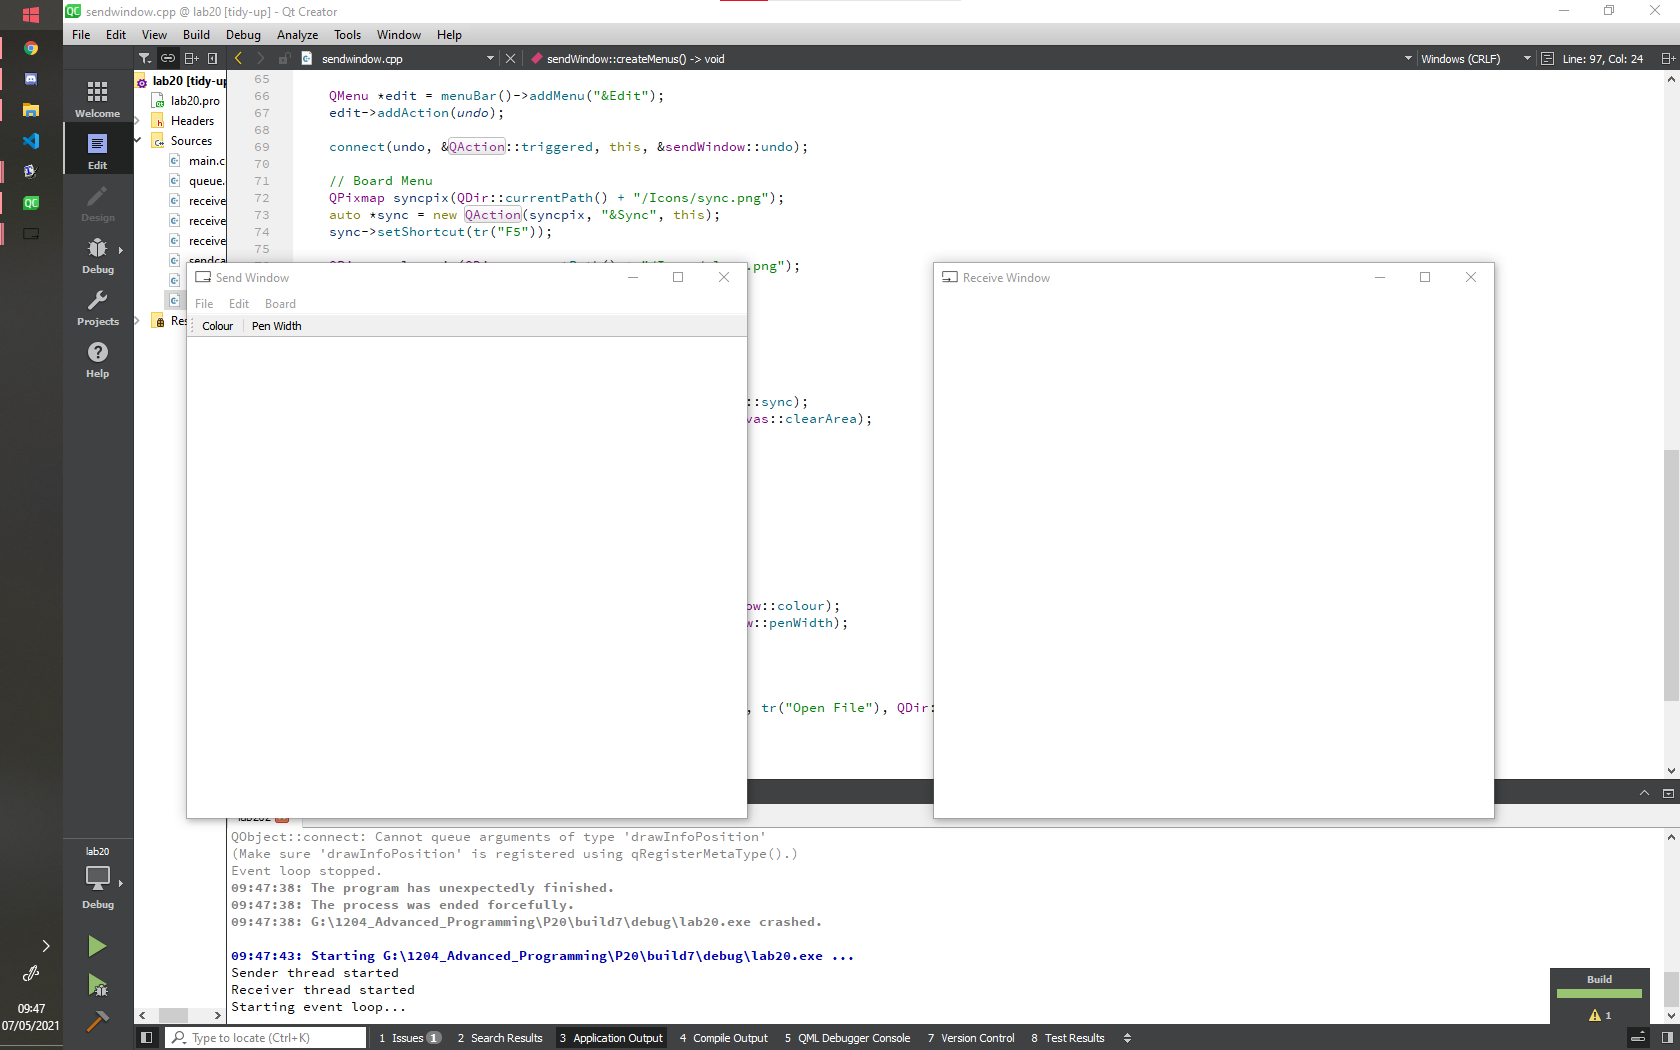
\includegraphics[width=\columnwidth]{./application.png}
		\caption{Send and receive windows when application is opened}
		\label{fig:app}
	\end{subfigure}
	\hfill
	\begin{subfigure}[t]{0.48\columnwidth}

		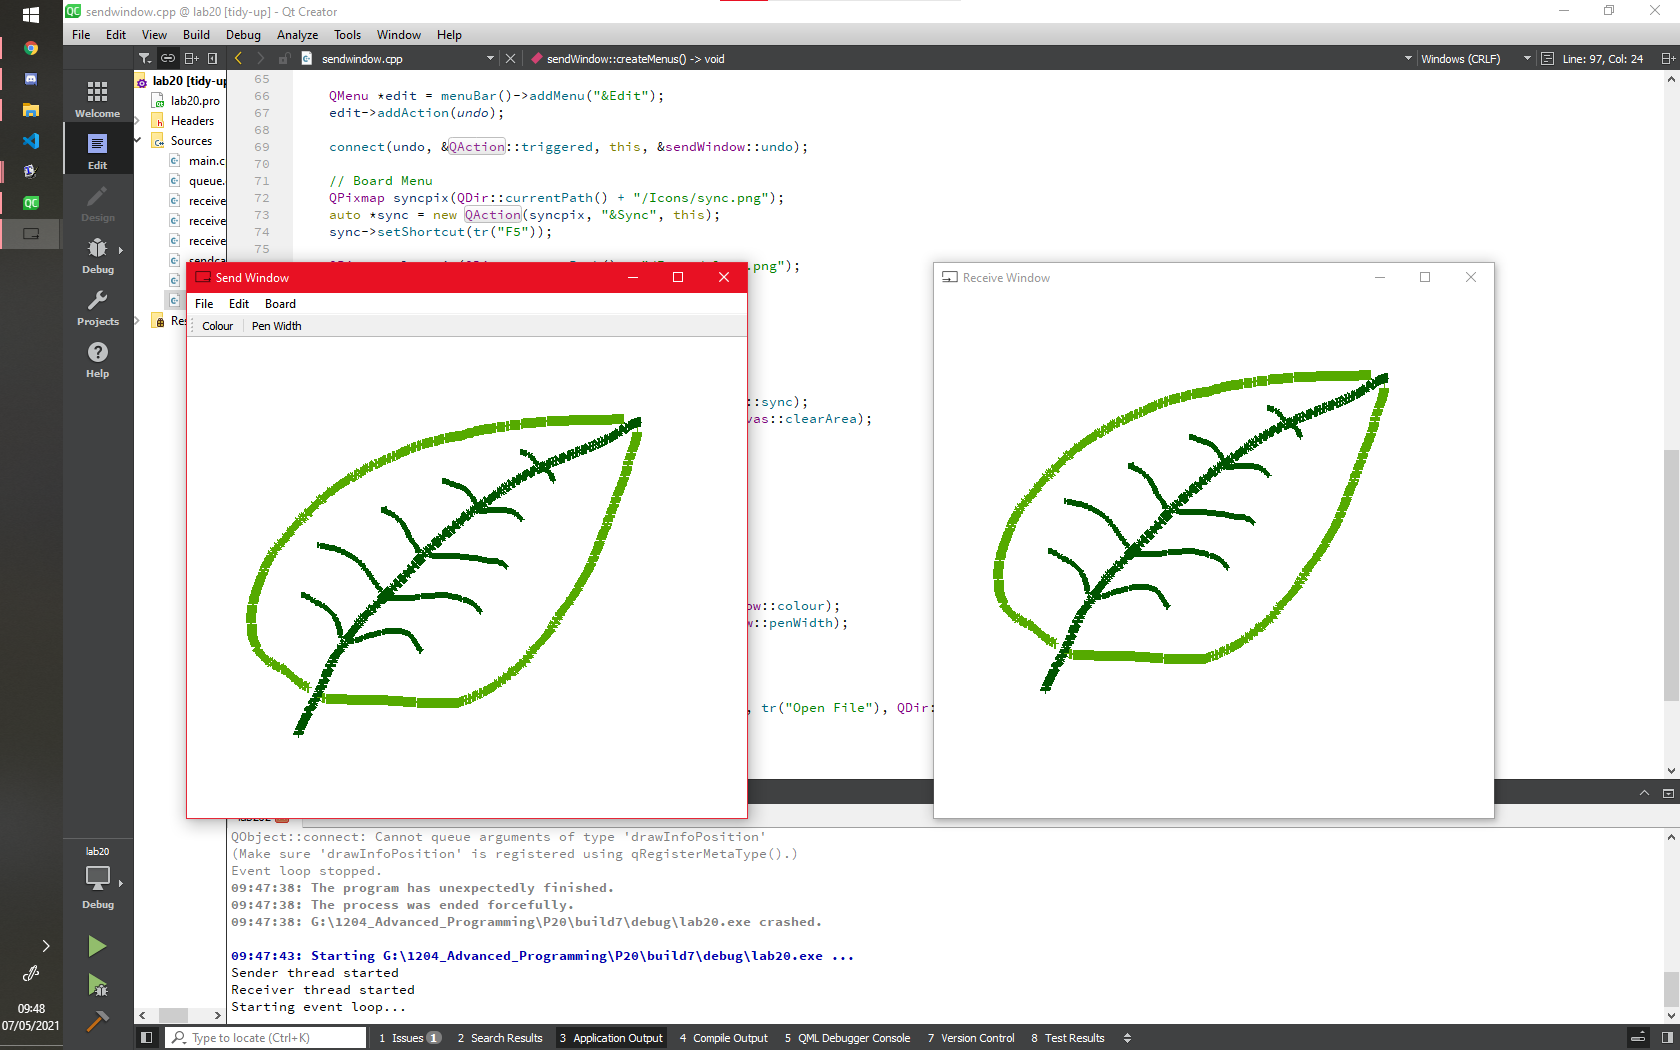
\includegraphics[width=\columnwidth]{./application drawing.png}
		\caption{Send and receive windows after drawing}
		\label{fig:app-drawing}
	\end{subfigure}
	\caption{Send and receive windows open on screen and allow drawing between them}
	\label{fig:application}
\end{figure}
\figsquish

\begin{figure}[H]
	\centering
	\begin{subfigure}[t]{0.32\columnwidth}

		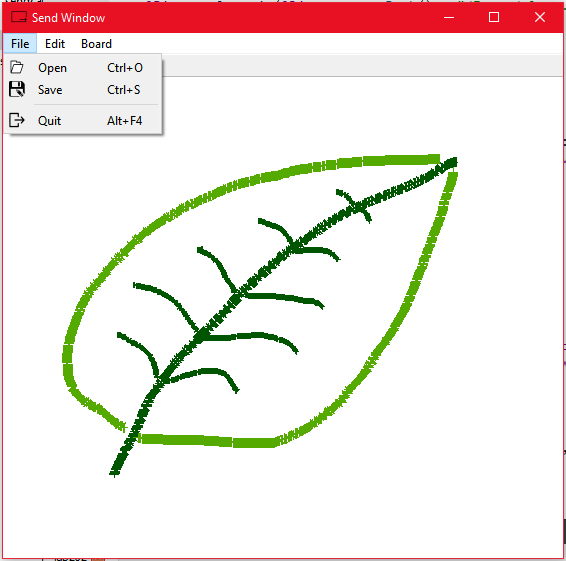
\includegraphics[width=\columnwidth]{./file.png}
		\caption{File Menu with  opening saving and closing}
		\label{fig:file}
	\end{subfigure}
	\hfill
	\begin{subfigure}[t]{0.32\columnwidth}

		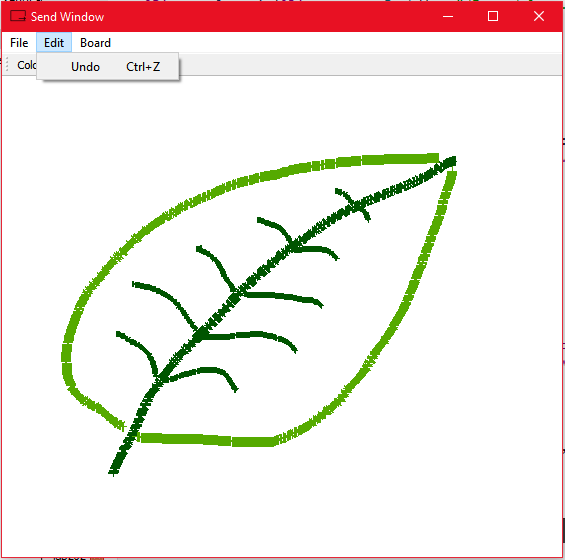
\includegraphics[width=\columnwidth]{./edit.png}
		\caption{Edit Menu with the undo functionality, redo was to be added later}
		\label{fig:edit}
	\end{subfigure}
	\hfill
	\begin{subfigure}[t]{0.32\columnwidth}

		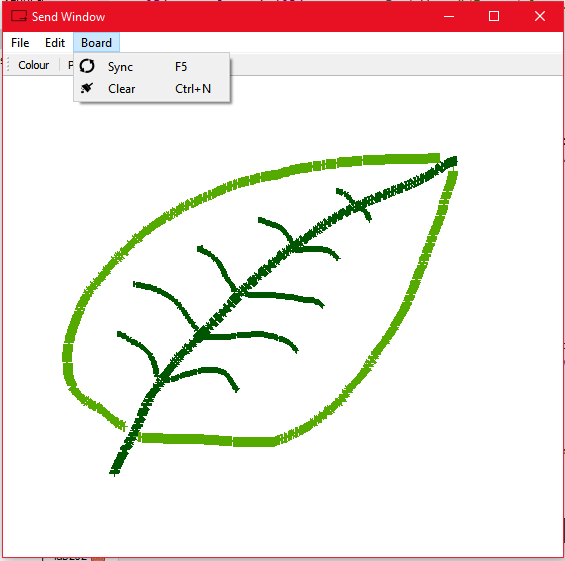
\includegraphics[width=\columnwidth]{./board.png}
		\caption{Board menu allows the screen to be cleared or windows to be synced}
		\label{fig:board}
	\end{subfigure}
	\caption{Menus allow the user to control the program}
	\label{fig:menus}
\end{figure}
\figsquish

\begin{figure}[H]
	\centering
	\begin{subfigure}[t]{0.48\columnwidth}

		
\includegraphics[width=\columnwidth]{./open.png}
		\caption{Open file dialog}
		\label{fig:open}
	\end{subfigure}
	\hfill
	\begin{subfigure}[t]{0.48\columnwidth}

		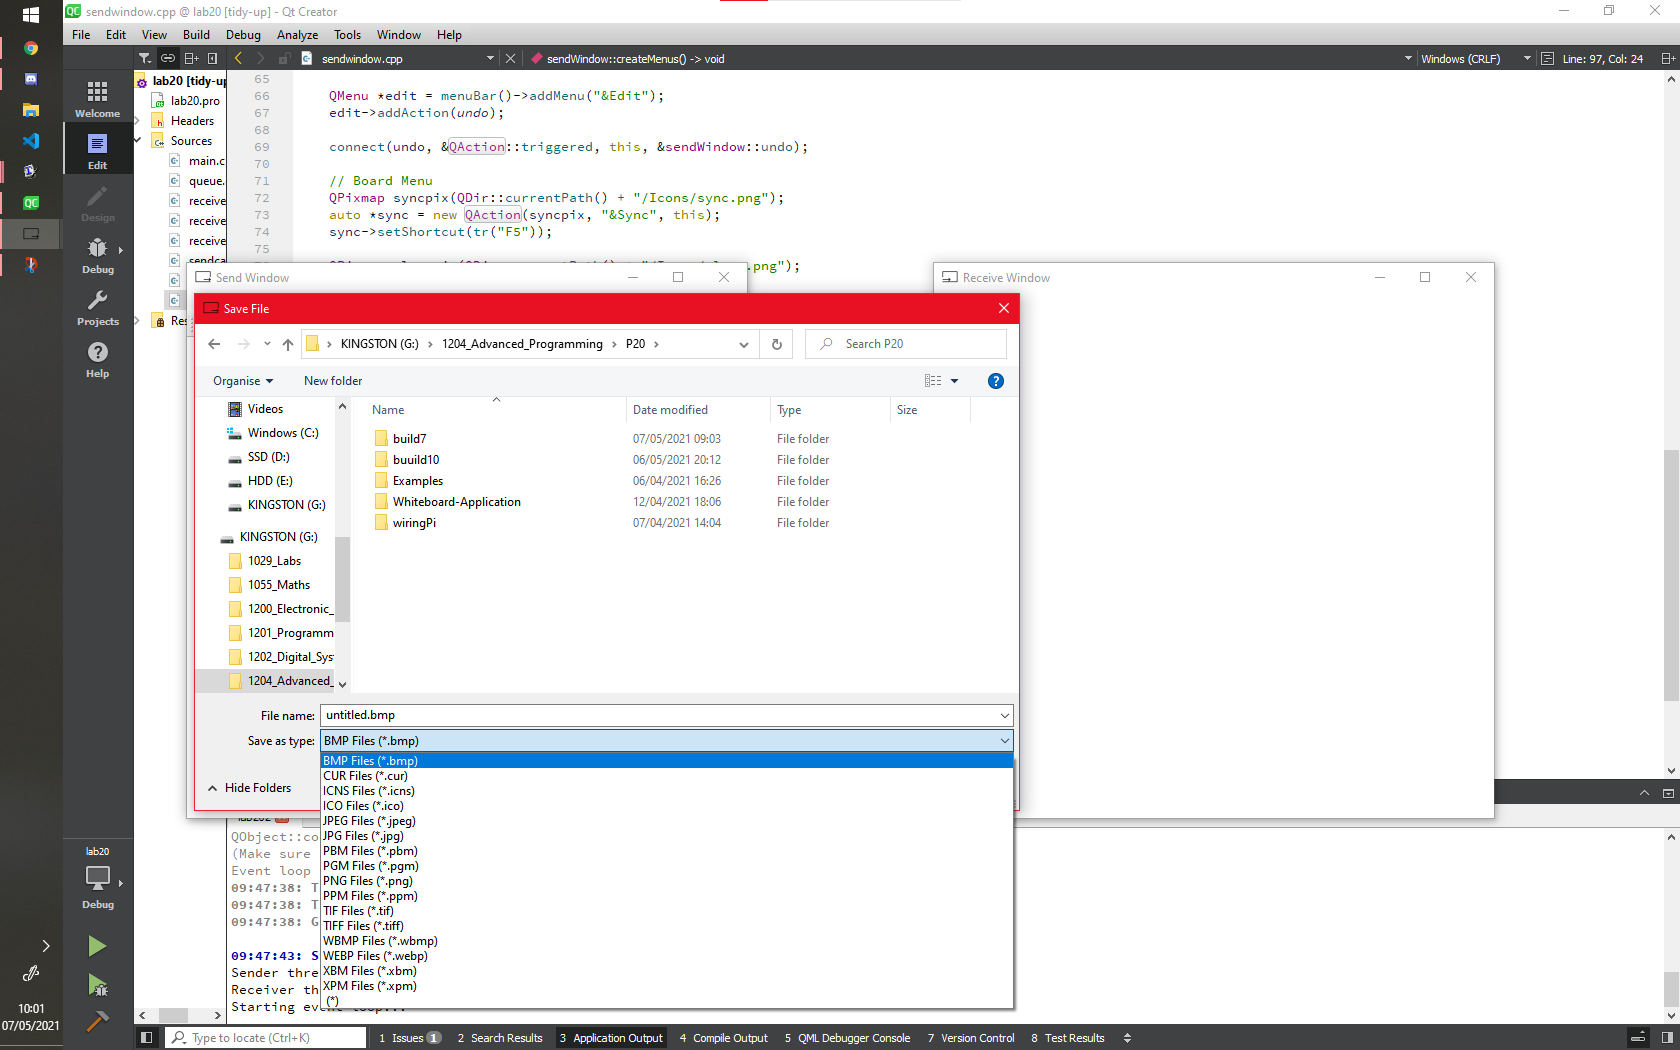
\includegraphics[width=\columnwidth]{./save.png}
		\caption{Save file dialog}
		\label{fig:save}
	\end{subfigure}
	\caption{File handling dialogs using QFileDialog}
	\label{fig:fileDialogs}
\end{figure}
\figsquish

\begin{figure}[H]
	\centering
	\begin{subfigure}[t]{0.48\columnwidth}

		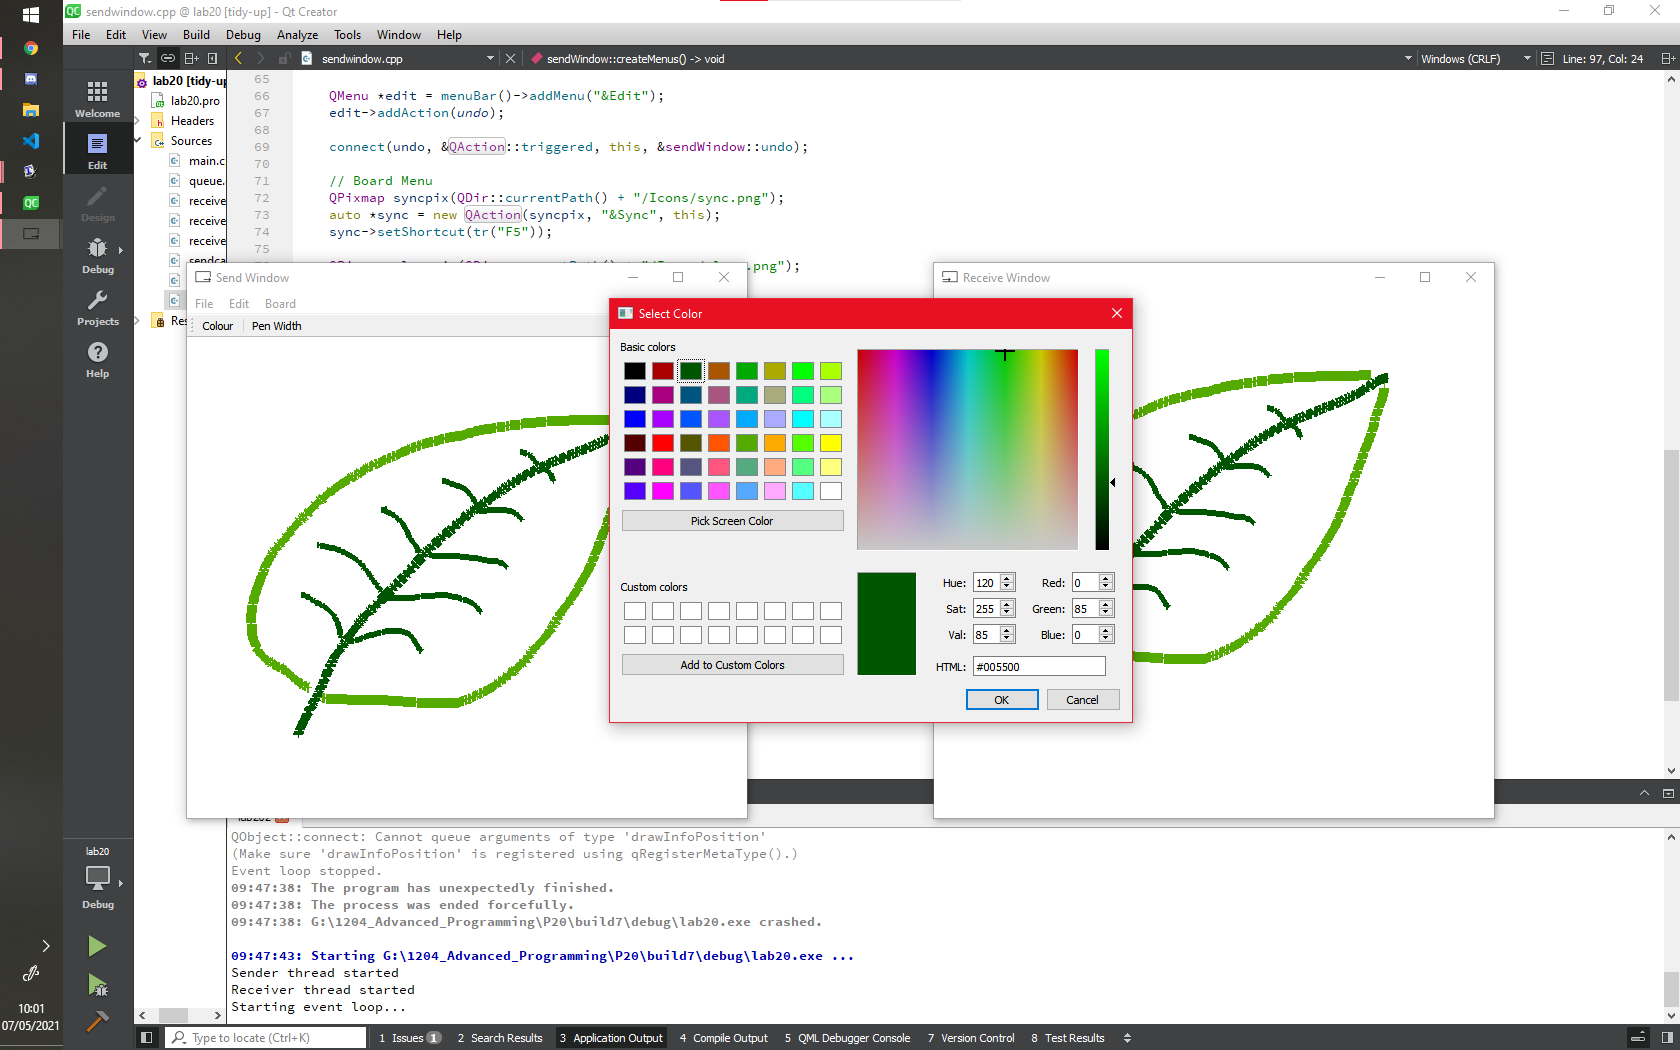
\includegraphics[width=\columnwidth]{./colour.png}
		\caption{Colour selection dialog box}
		\label{fig:colour}
	\end{subfigure}
	\hfill
	\begin{subfigure}[t]{0.48\columnwidth}

		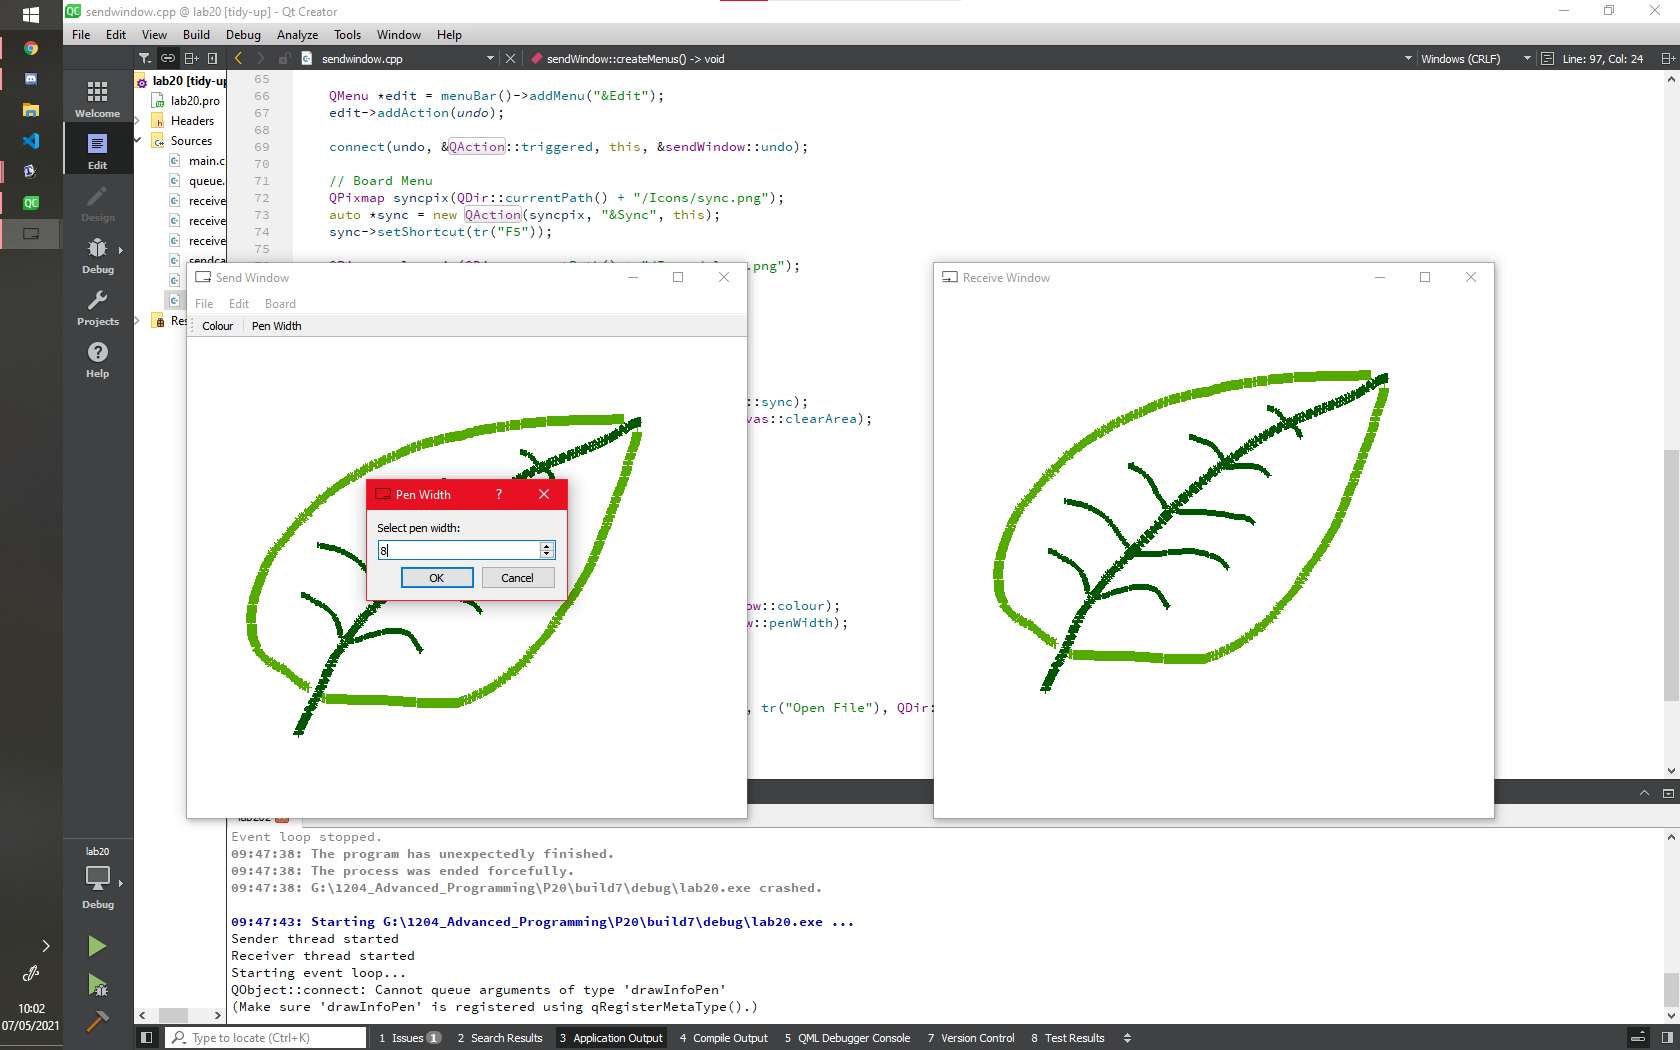
\includegraphics[width=\columnwidth]{./width.png}
		\caption{Pen width control dialog box}
		\label{fig:width}
	\end{subfigure}
	\caption{Dialog boxes to control the QPen characteristics}
	\label{fig:drawDialogs}
\end{figure}
\figsquish


\section{Discussion}
\subsection{GUI - Send and Receive Windows}
The send and receive window were initiasised in a relatively standard way. However, the use of getting the screen geometry information allowed the program to scale better across different users. This program was written on a 1080p monitor, a visually pleasing size on this display is likely to be too small for any end user that has a 2160p monitor.

The send window was well featured with the ability to change the pen and, save and load the canvas as images. This gave the send window a feature set similar to a simple paint application. This is a good range of utility for a whiteboard application to be able to do.

In addition, the layout of features is similar in format to other contemporary desktop applications. This makes the program intuitive and easy to use as any user will know where to look for the tool that they are looking for.

The addition of an undo feature is a nice quality of life feature that makes the application more pleasurable to use. This was implemented by snapshoting the draw area image every time the mouse was released. The lack of a redo feature is apparent. The redo functionality could be implemented using a lot of the same code as the undo feature.

\subsection{The Serialise and Deserialise Drawing Commands}
The method to serialise and deserialise the drawing commands is a relatively common method in C++ programming. This makes it a reliable method as it is unlikely to break from a new version of Qt being used. In addition, this means that if there are found to be any issues they are likely to be well documented reducing the time needed to fix the issue. However, not using any features from Qt or Vector means that the code is not as succinct as it otherwise may have been.

Furthermore, the use of the drawInfoPosition struct is another instance of bloat in the code, as any conversion from QPoint or QPen could be carried out at the serialisation stage. This is the result of previous implementation of drawing and could be streamlined. Although bloated, this does not apppear to have anylarge detrement to the code itself.

\subsection{The Send and Receive Threads}
The send and receive threads successfully initialised inside the instances of the canvases. The canvas was able to communicate with the thread using signals and slots. This meant that information could easily be passed down into the thread to go to the receive window.

The use of QMutex was a useful way of ensuring that functions were thread safe. QMutex meant that a lot of the the complicated threading issues were conveniently handled by the program. This removed a level of risk from a race condition occuring.

The lack of a functioning queue was a severe detrement to this project. Lacking a queue there was no common object that the send and receive threads could communicate through. This made the threads practically pointless as they were unable to fulfill the communication they were there to enable.

Althought the implemented queue appeared to be thread safe and controlled the items put onto and pulled off of it correctly the inability to compile it with the rest of the program suggests that there is likely a problem with the use of QMutex in the class.

\subsection{Communicaiton Protocol Using Booleans}
Parity calculations are a useful way of checking that the received information has been received correctly. The use of parity meant that the communication between threads would have been consided a half-duplex protocol.

The parity calculations used in the implemented protocol are relatively simple and do not accaount for two bit flips in a signal. Nor does the parity method used in this protocol tell you what part of the information has an error. However, this is likely to be sufficient for the communication between two devices with GPIO as there is likely to be very little noise on the short wired connection.

The lack of a functioning queue was again an issue. As there was no shared class between the threads so they were unable to flip shared bits, emulating the role of a GPIO pin.

\section{Conclusion}
A Whiteboard chat application was successfully created. However, it did not acheive all the aims that it had been set.

The created application had the basic feature range of a simple paint application. It had an intuitive UI that took full advantage of the Qt libraries, and was easy to use. The program used a simplex communication protocol between the send canvas and a receive canvas that would transmit the draw information.

The application attempted to send serialised versions of the commands through send and receive threads. Although the threads were created successfully the communication between them was nto successfully implemented.

The progress of the application was severly limited by the lack of a thread safe queue that the send and receive threads could communicate through. This prevented a half-duplex communication protocol being implemented as there was no common class between the threads.


%%%%%%%%%%%%%%%%%%%%%%%%%%%%%%%%%%
% BIBLIOGRAPHY
%%%%%%%%%%%%%%%%%%%%%%%%%%%%%%%%%%
\nocite{*} % show all references even without citation
% to cite use "bla bla"~\cite{ref_label} -> "bla bla" [1]
\bibliographystyle{IEEEtran}
% IEEEabrv abbreviates journal titles in accordance to IEEE standards 
\bibliography{IEEEabrv,mybib}

\end{multicols*}
\end{document}
